\section{cal\_\-table.h File Reference}
\label{cal__table_8h}\index{cal_table.h@{cal\_\-table.h}}


This graph shows which files directly or indirectly include this file:\begin{figure}[H]
\begin{center}
\leavevmode
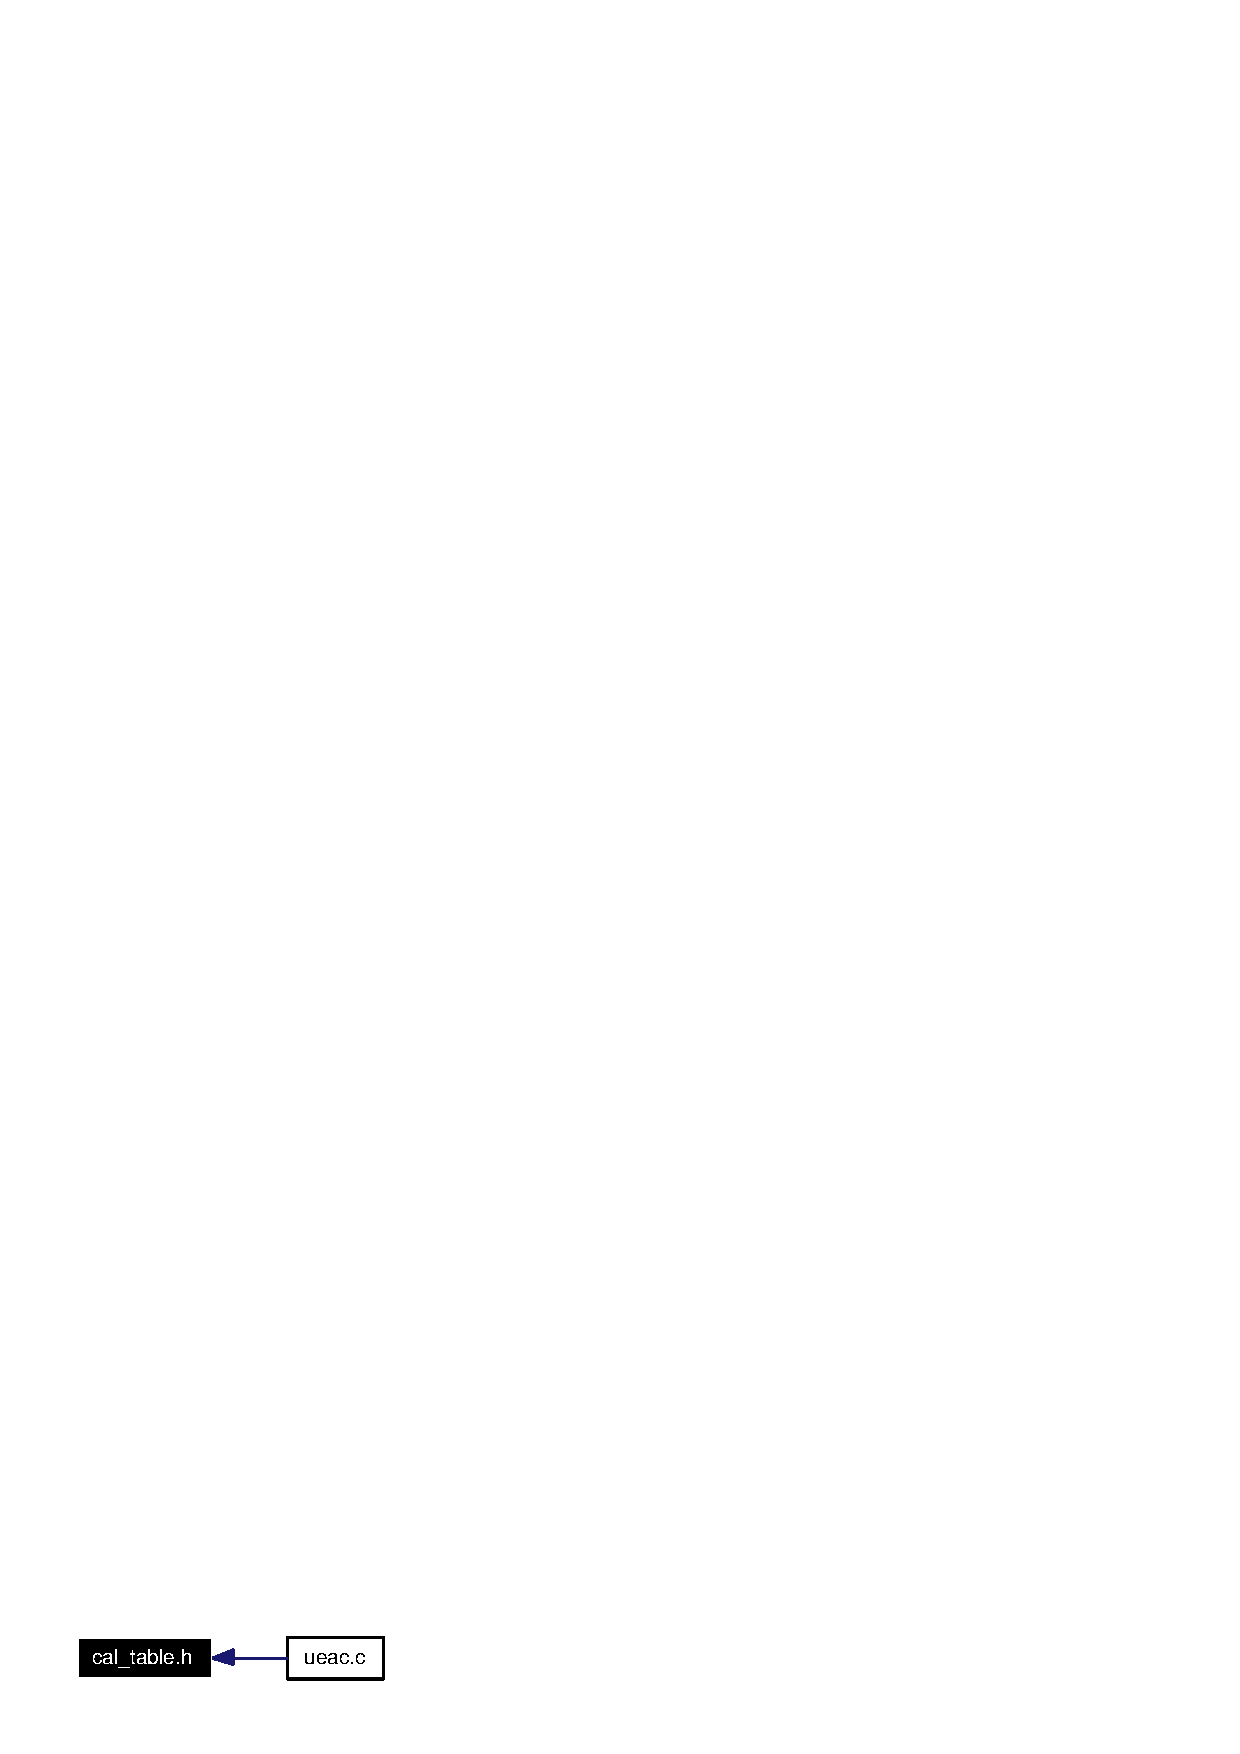
\includegraphics[width=92pt]{cal__table_8h__dep__incl}
\end{center}
\end{figure}
\subsection*{Variables}
\begin{CompactItemize}
\item 
const short {\bf dac\_\-translation} [$\,$]
\end{CompactItemize}


\subsection{Variable Documentation}
\index{cal_table.h@{cal\_\-table.h}!dac_translation@{dac\_\-translation}}
\index{dac_translation@{dac\_\-translation}!cal_table.h@{cal\_\-table.h}}
\subsubsection{\setlength{\rightskip}{0pt plus 5cm}const short {\bf dac\_\-translation}[$\,$]}\label{cal__table_8h_a0}




Definition at line 45 of file cal\_\-table.h.

Referenced by current\_\-output\_\-calibration(), and write\_\-current().